%

% File final_report.tex
%
%% Based on the style files for ACL 2020, which were
%% Based on the style files for ACL 2018, NAACL 2018/19, which were
%% Based on the style files for ACL-2015, with some improvements
%%  taken from the NAACL-2016 style
%% Based on the style files for ACL-2014, which were, in turn,
%% based on ACL-2013, ACL-2012, ACL-2011, ACL-2010, ACL-IJCNLP-2009,
%% EACL-2009, IJCNLP-2008...
%% Based on the style files for EACL 2006 by 
%%e.agirre@ehu.es or Sergi.Balari@uab.es
%% and that of ACL 08 by Joakim Nivre and Noah Smith

\documentclass[10pt,letter]{article}
\usepackage[hyperref]{acl2020}
\usepackage{times}
\usepackage{latexsym}
\usepackage{listings}
\usepackage{minted}
\usepackage{amsmath}
\usepackage{fancyvrb}
\usepackage{subcaption}
\usepackage{makecell}
\usepackage{placeins}
\usepackage{hyperref}
\usepackage{graphicx}
\graphicspath{ {./} }
\renewcommand{\UrlFont}{\ttfamily\small}
\usepackage[
    %backend=biber, 
    natbib=true,
    style=numeric,
    sorting=none
]{biblatex}
\addbibresource{citations.bib}

% This is not strictly necessary, and may be commented out,
% but it will improve the layout of the manuscript,
% and will typically save some space.
\usepackage{microtype}
\usepackage[T1]{fontenc}

\aclfinalcopy % Uncomment this line for the final submission
%\def\aclpaperid{***} %  Enter the acl Paper ID here

%\setlength\titlebox{5cm}
% You can expand the titlebox if you need extra space
% to show all the authors. Please do not make the titlebox
% smaller than 5cm (the original size); we will check this
% in the camera-ready version and ask you to change it back.

\newlength{\mintednumbersep}
\AtBeginDocument{%
  \sbox0{\tiny00}%
  \setlength\mintednumbersep{\parindent}%
  \addtolength\mintednumbersep{-\wd0}%
}

\newcommand\BibTeX{B\textsc{ib}\TeX}

\newenvironment{tight_enumerate}{
\begin{enumerate}
\setlength{\itemsep}{0pt}
\setlength{\parskip}{0pt}
}{\end{enumerate}}

\newenvironment{tight_itemize}{
\begin{itemize}
\setlength{\itemsep}{0pt}
\setlength{\parskip}{0pt}
}{\end{itemize}}

\title{Music Source Separation With Different Time-Frequency Representations}

\author{Sevag Hanssian \\
  McGill University \\
 \texttt{sevag.hanssian@mail.mcgill.ca} \\
 \texttt{sevagh@protonmail.com}}

\date{}

\begin{document}
\maketitle

%%%%%%%%%%%%%%
% ABSTRACT			%
%%%%%%%%%%%%%%
\begin{abstract}
	\citet{fitzgerald1} presented an algorithm for separating a musical mix into harmonic and percussive components by applying masks on the short-time Fourier transform (STFT). \citet{driedger} created an iterative variant using a large window for the harmonic separation and a small window for the percussive separation. \citet{fitzgerald2} introduced the constant-Q transform (CQT) to also separate the vocal component. The field of wavelets has produced similar algorithms for tonal/transient separation, such as \citet{tfjigsaw}'s Jigsaw Puzzle. A survey of different time-frequency representations used for harmonic/percussive/vocal source separation is proposed. They will be implemented and evaluated in MATLAB, and the best performers will be combined in a hybrid algorithm to compare with a state-of-the-art neural network.
\end{abstract}

%%%%%%%%%%%%%%
% INTRODUCTION		%
%%%%%%%%%%%%%%
\section{Introduction}
\label{sec:intro}

In music source separation, a mixed song is split into its constituent components, or sources. There are different types of source separation; in this report, two cases will be considered:

\begin{tight_enumerate}
	\vspace{-0.5em}
	\item
		Harmonic/percussive source separation (HPSS)
	\item
		Harmonic/percussive/vocal source separation
\end{tight_enumerate}

There are other terms used to indicate similar algorithms. For example, \citet{bayarres} refers to harmonic/percussive source separation as steady-state/transient source separation. In the wavelet domain, the same algorithm is called tonal/transient separation (\cite{tfjigsaw}, \cite{wmdct}).

\subsection{Methods based on the STFT and CQT}

Harmonic (or steady-state, or tonal) sounds are narrowband (contain few well-defined frequencies) and steady (maintain the same frequency components over long periods of time), while percussive sounds  are broadband (contain most of the frequency spectrum) and transient (fast attack and decay). These manifest as horizontal and vertical lines respectively in the short-time Fourier transform. \citet{fitzgerald1} applied a median filter in the vertical and horizontal directions to estimate the harmonic and percussive components, and used these to compute soft masks. The masks were then applied to the original STFT and inverted to create the harmonic and percussive signals. An example can be seen in Figure \ref{fig:fitz1}.

\begin{figure}[ht]
	\centering
	\vspace{-0.8em}
	\subfloat[Mixed signal]{{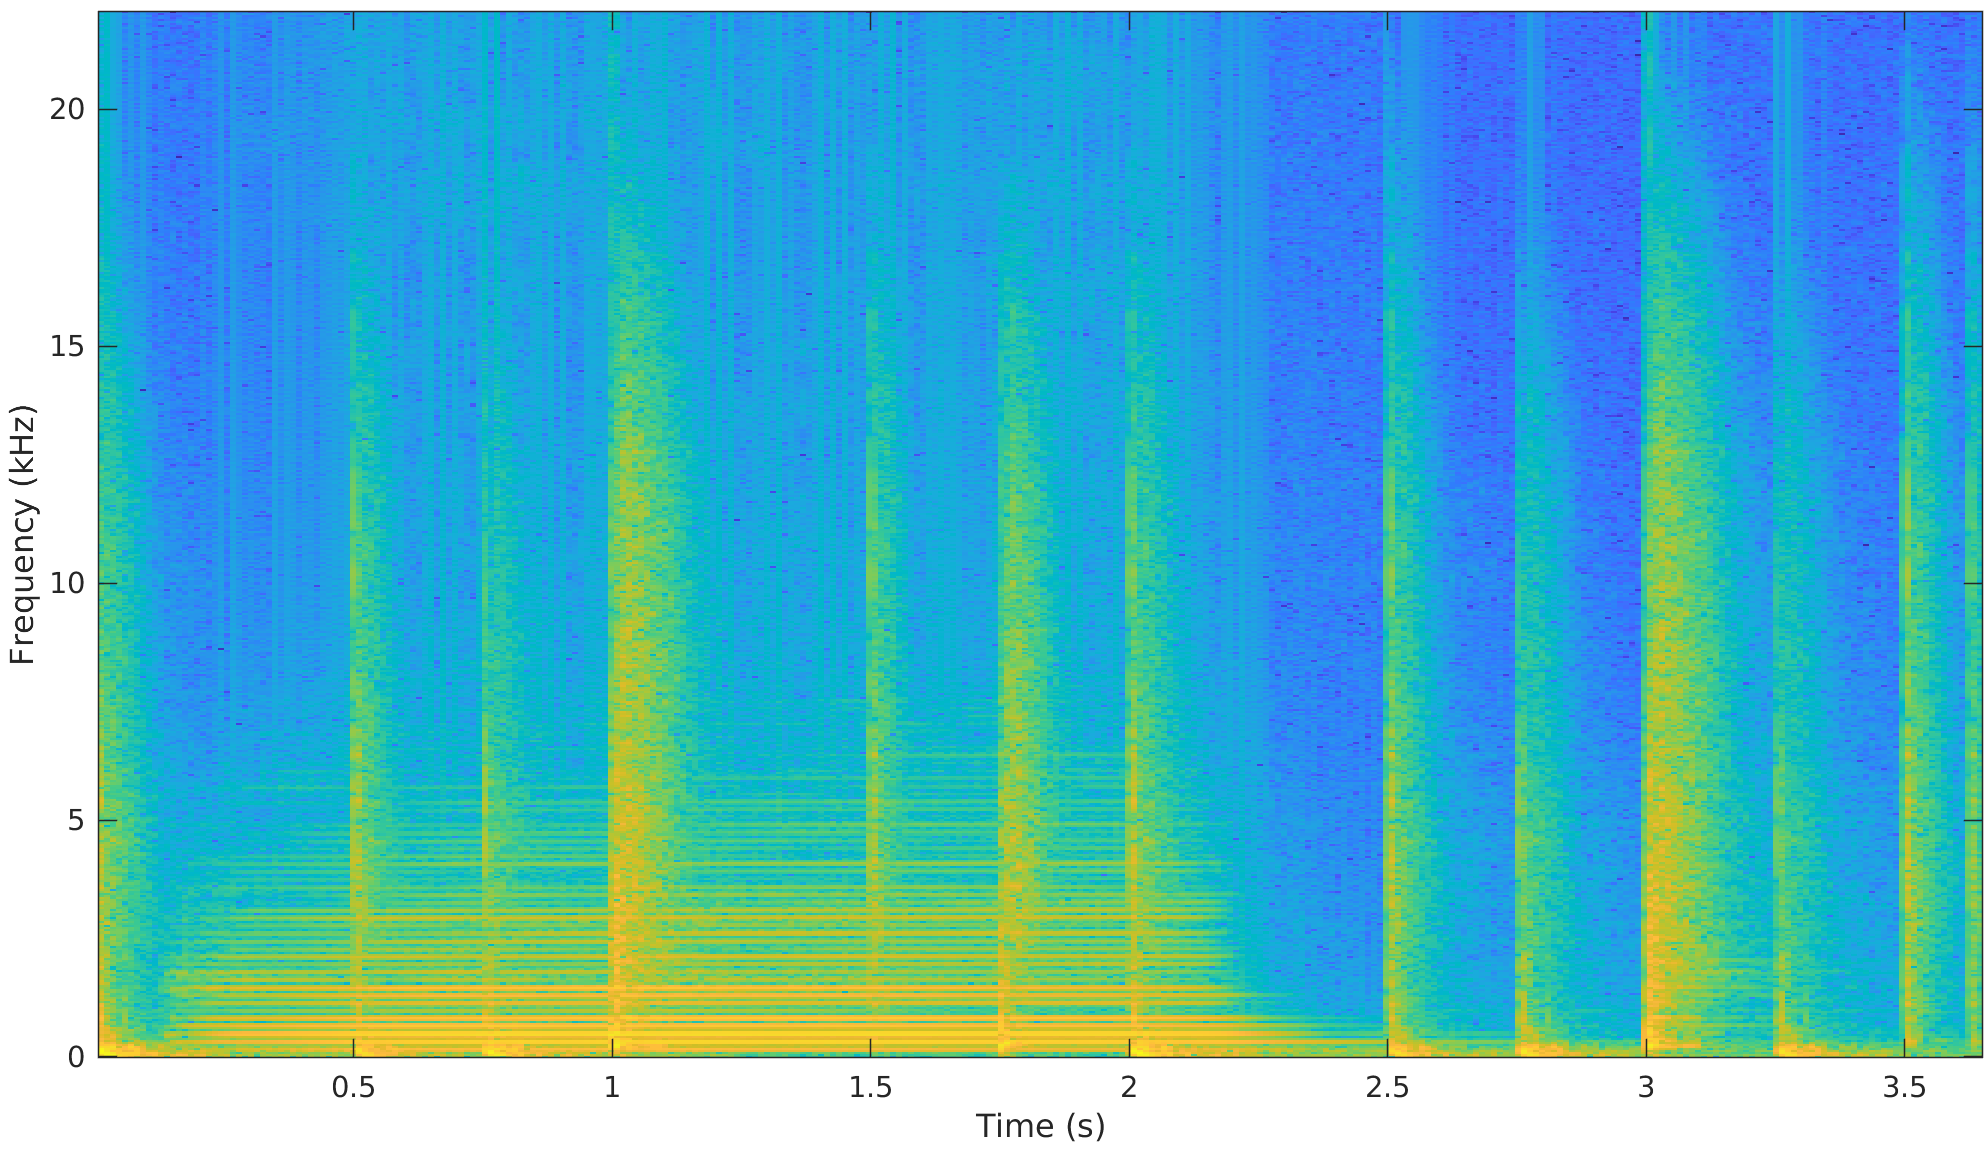
\includegraphics[width=4cm]{./mixedspecgram.png} }}
	\\
	\subfloat[Percussive separation]{{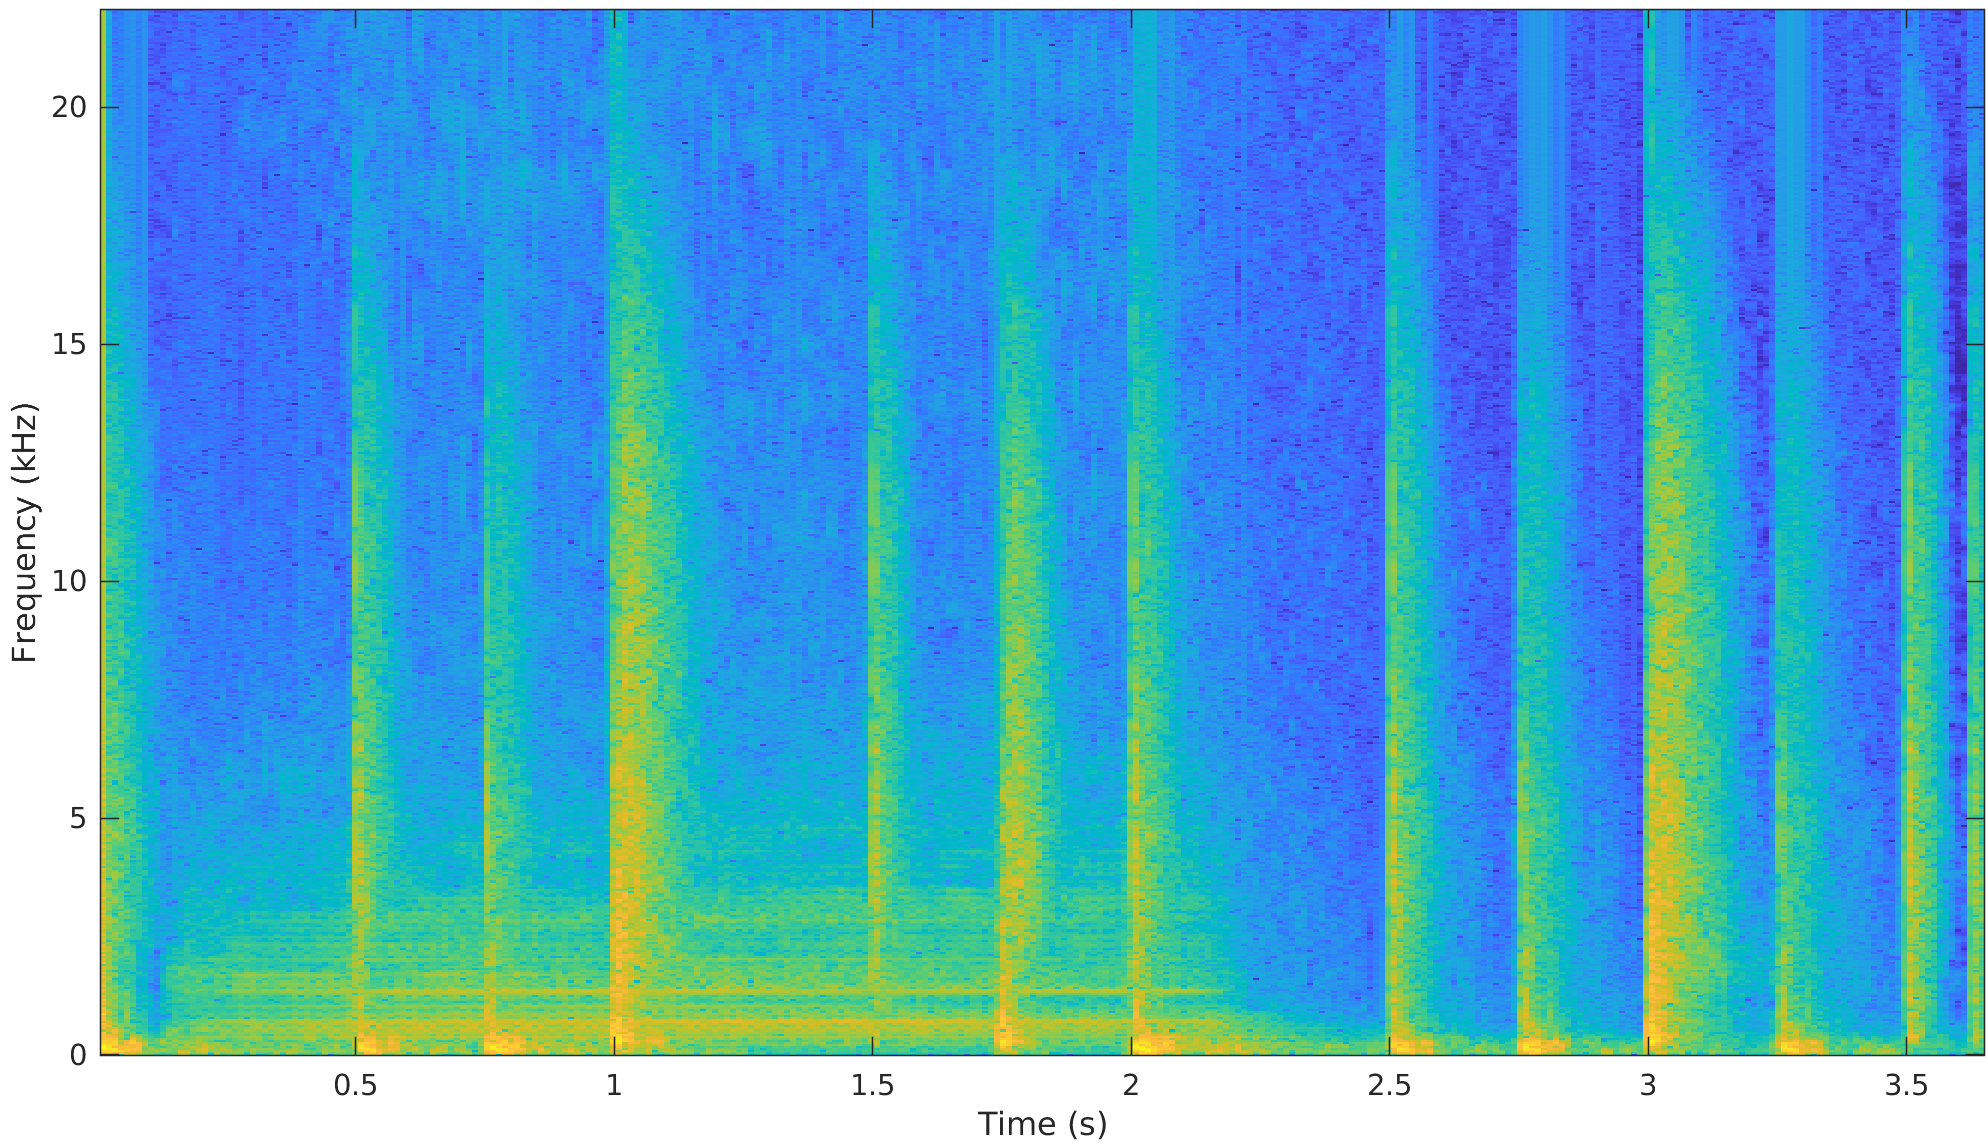
\includegraphics[width=4cm]{./perc_soft.png} }}
	\subfloat[Harmonic separation]{{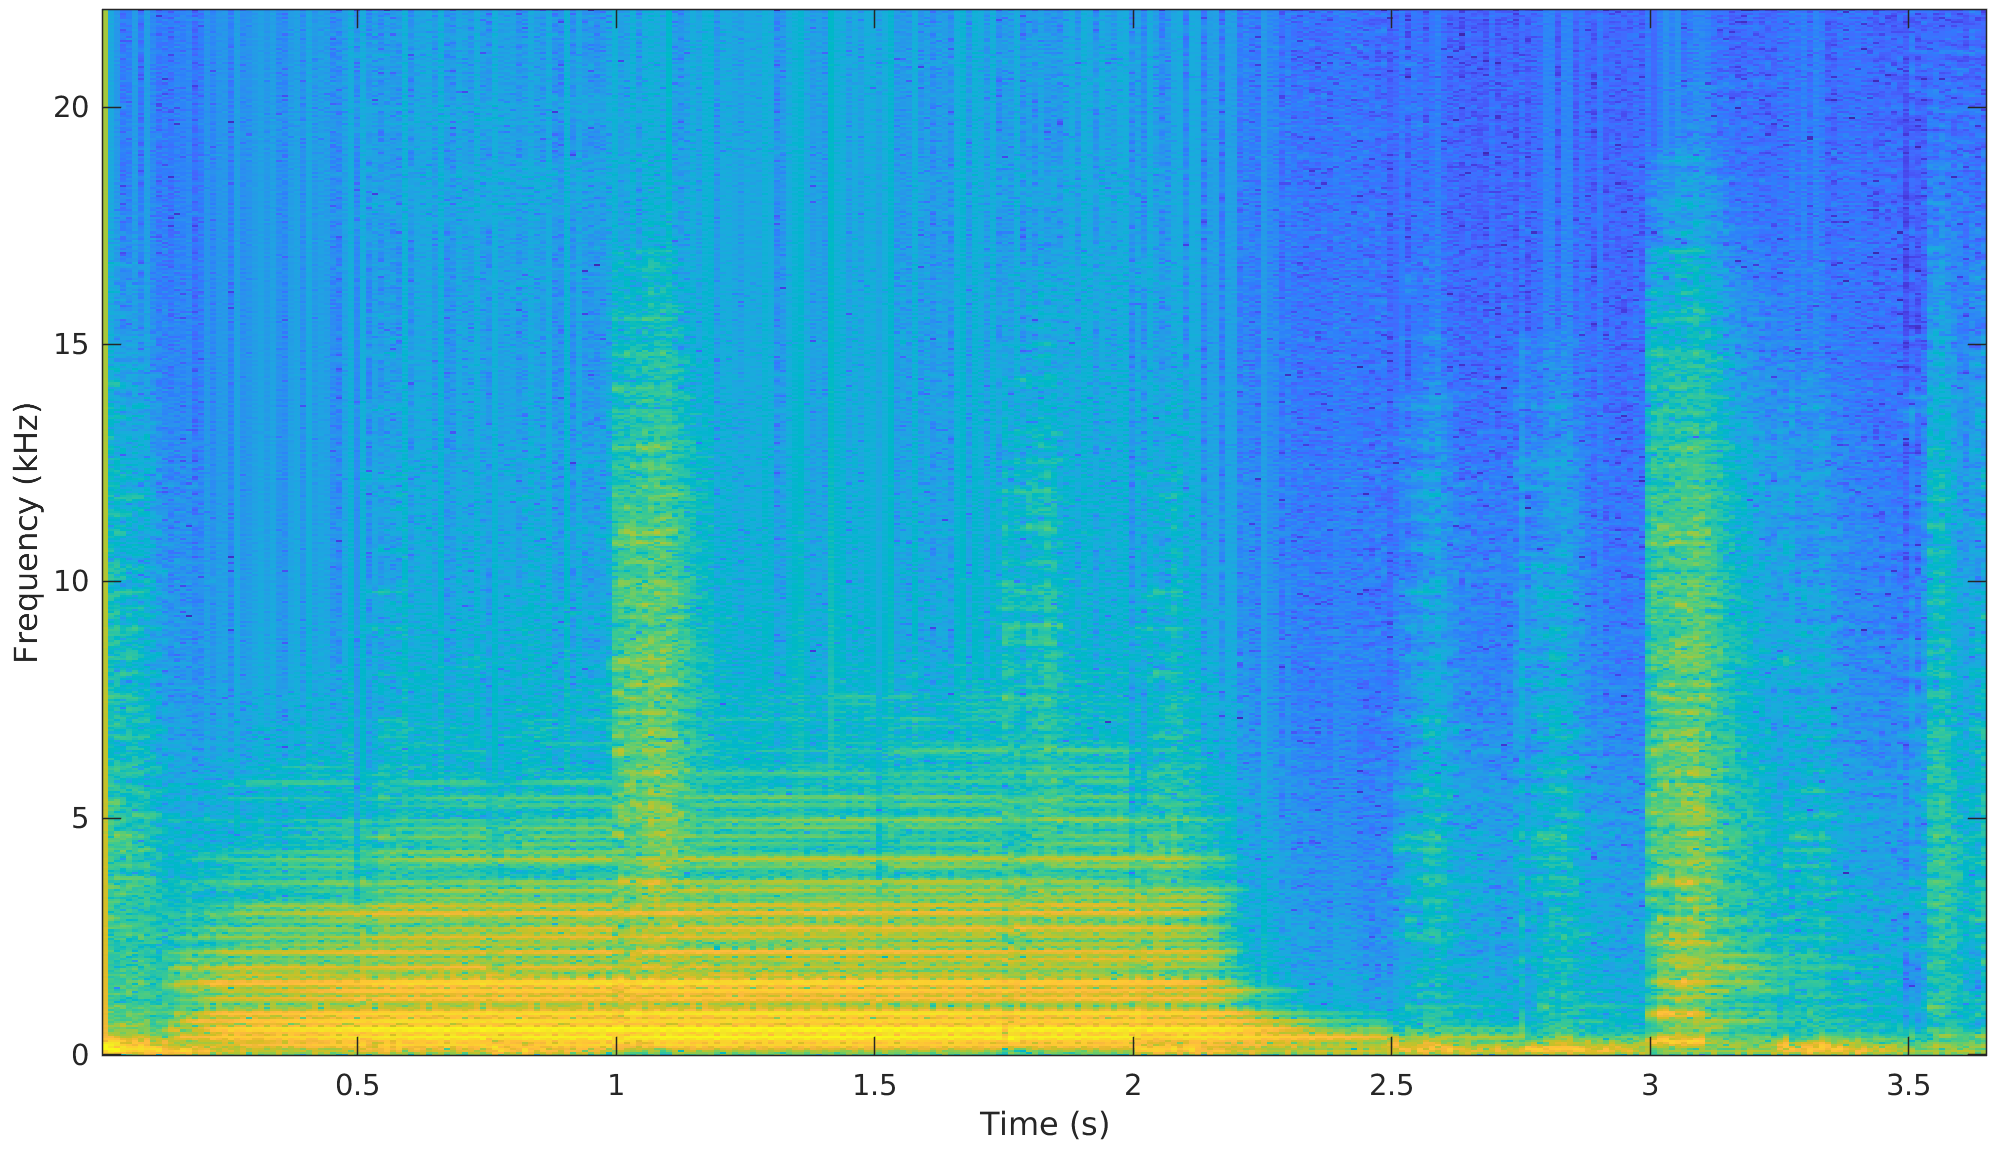
\includegraphics[width=4cm]{./harm_soft.png} }}
	\caption{Example of median-filtering HPSS}
	\label{fig:fitz1}
\end{figure}

\citet{driedger} replaced the soft mask with a binary/hard mask, and also introduced a two-pass variant. The STFT with a large window size in the first pass separates the harmonic components with higher frequency resolution, and the STFT with a small window size in the second pass separates the percussive component with higher time resolution.

\citet{fitzgerald2} created a similar iterative variant, using soft masks, a large window STFT in the first pass for harmonic separation, and a small window STFT in the second pass for percussive separation. Additionally, they noted that if they replaced the small-window STFT with the constant-Q transform in the second pass, they obtained a separation of the human singing voice.

In sum, from the above papers, we can consider two generalized frameworks for harmonic/percussive (and optionally vocal) source separation with masking and median filtering of either the STFT and CQT, considering the one-pass and two-pass variants separately. In each, we can substitute different window sizes of STFT (128--16384), and the CQT with different bins per octave (12--96) to test the results.

\subsection{Methods based on wavelets}

Two algorithms will be considered from the wavelet domain, which are implemented in the Large Time-Frequency Analysis toolbox (\cite{ltfat}).

%%%%%%%%%%%%%%
% THEORY     %
%%%%%%%%%%%%%%
\section{Theory}
\label{sec:theory}

\subsection{Gabor dictionaries}

\subsection{STFT and CQT}

\subsubsection{Time-frequency resolution}

\subsubsection{Median filtering}

\subsection{TF Jigsaw}

\subsection{Group lasso shrink}

%%%%%%%%%%%%%%%
% METHODOLOGY %
%%%%%%%%%%%%%%%
\section{Methodology}
\label{sec:methodology}

\subsection{Objective measures}

The SigSep (\href{https://sigsep.github.io/}{https://sigsep.github.io/}) community, borrowing from the methodology of Signal Separation Evaluation Campaign (SISEC), uses the MUSDB18 dataset \cite{musdb18} (or the HQ, high-quality, equivalent \cite{musdb18-hq}), and uses the BSS (Blind Source Separation) Eval (\cite{bss}) objective measure for separation quality.

The authors of BSS released an improved version that matches better with subjective human evaluations, which they called the PEASS (Perceptual Evaluation methods for Audio Source Separation) Toolkit (\cite{peass}), based on PEMO-Q (\cite{pemoq}). The PEASS Toolkit for MATLAB (\cite{peassmatlab}) conveniently includes all 3 measures: PEASS, PEMO-Q, and BSS. Each of these consist of 4 metrics:

\begin{tight_itemize}
\vspace{-0.5em}
\item
	\textbf{Target:} measure of desired sound in the separation. TPS (Target Perceptual Score) in PEASS, ISR (source Image to Spatial distortion Ratio) in BSS, qTarget in PEMO-Q.
\item
	\textbf{Interference:} measure of undesired sounds in the separation. IPS (Interference Perceptual Score) in PEASS, SIR (Signal to Interference Ratio) in BSS, qInterf in PEMO-Q.
\item
	\textbf{Artifacts:} measure of artifacts in the separation. APS (Artifact Perceptual Score) in PEASS, SAR (Signal to Artifacts Ratio) in SAR, qArtif in PEMO-Q.
\item
	\textbf{Global:} a global score for the previous three. In PEASS, this is OPS (Overall Perceptual Score). In BSS, this is SDR (Signal to Distortion Ratio). In PEMO-Q, this is qGlobal.
\end{tight_itemize}

\citet{beassvpeass} make the recommendation to use PEASS for music separation evaluation, noting the importance of perception in music applications. They also recommend to evaluate algorithms based on their separate target, interference, and artifact scores, noting that the global measure of OPS (for PEASS) and SDR (for BSS) have an uncertain relation to the three constituent scores. The choice in this paper is to use three measures from the PEASS for all performed evaluations:
\begin{tight_enumerate}
	\vspace{-0.5em}
	\item
		\textbf{TPS} (Target Perceptual Score)
	\item
		\textbf{APS} (Artifact Perceptual Score)
	\item
		\textbf{IPS} (Interference Perceptual Score)
\end{tight_enumerate}

\subsection{Evaluated music}

A limited subset of MUSDB18-HQ was evaluated, or 5 total minutes of music, consisting of 4 segments of 15 seconds duration taken from 5 separate tracks. One data set was prepared for harmonic/percussive separation evaluation (vocals omitted from the mix), and one data set for harmonic/percussive/vocal evaluation (vocals are present). The evaluation was limited to 5 minutes of music since the PEASS measure is computationally expensive.

MUSDB18-HQ contains stems (.wav files per component, e.g., drum.wav, vocal.wav, bass.wav) from a collection of permissively licensed music, specifically intended for recording, mastering, mixing (and in this case, ``de-mixing'') research. The songs are split across train and test sets. Since the final comparison of this paper will consider a neural network model which was trained on MUSDB18, the evaluation data is taken from the test set -- if we took it from the training set, the neural network could overfit and overperform.

\subsection{Evaluation format}

Due to the large number of algorithms and configurations that will be evaluated, introducing them all at the same time will be overwhelming, and will make it difficult to form conclusions.

The proposed format will be an elimination tournament, similar to sports tournaments. Starting from the simplest one-pass algorithm for harmonic/percussive source separation, we can perform evaluations to form intermediate conclusions:

\begin{tight_itemize}
\vspace{-0.5em}
\item
	Is the STFT or CQT better for harmonic/percussive source separation
\item
	Which window size of STFT (out of 128, 256, 1024, 2048, 4096, 16384), or which bins-per-octave of CQT (12, 24, 48, 96), performs best
\item
	Which of soft or hard masking performs best
\end{tight_itemize} 

From these, we can move on to two-pass variants, by using the conclusions from the previous evaluation. Next, we can evaluate the wavelet-based methods with different configurations. After the harmonic/percussive evaluations are done, we can introduce vocal separation, and repeat.

The final goal is to combine the best performers to create optimal ``hybrid'' algorithms for each task: HPSS and harmonic/percussive/vocal separation. At the last stage, the optimal hybrids will be compared to Open-Unmix (\cite{umx}). Open-Unmix is an deep-learning-based music source separation system which achieves near state-of-the-art results. It is fully open-source, and was intended to be a reference and benchmark in the field of signal separation.

\subsection{Mixed Python/MATLAB testbench}

%%%%%%%%%%%%%%%%%%%%%%%%%%
% ELIMINATION TOURNAMENT %
%%%%%%%%%%%%%%%%%%%%%%%%%%
\section{Elimination tournament}
\label{sec:elim}

\textbf{N.B.:} as a shorthand, STFT with window size X will be referred to as STFT-X, and CQT with bins-per-octave X will be referred to as CQT-X. For example, CQT-96 is a CQT with 96 bins-per-octave, and STFT-2048 is an STFT with window size 2048.

\subsection{Harmonic/percussive source separation}

The first task is harmonic/percussive source separation. The mixtures are combined from the instrument stems (excluding vocals). The evaluation is performed on 5 minutes of music from MUSDB18-HQ, as was mentioned. The results are displayed as colored heatmaps, where green is the best result and red is the worst. This enables a quick visual verification of the best performers.

\subsubsection{One-pass algorithms}

The first and original median-filtering HPSS algorithm with soft masks was introduced by \citet{fitzgerald1}. The modification introduced by \citet{driedger} uses hard masks (the same paper contains the two-pass variant, which will be discussed later). Pseudocode for both algorithms is shown in Listing \ref{code:onepasspseudo}.

\begin{listing}[h]
\setlength\partopsep{-\topsep}
\begin{minted}[numbersep=\mintednumbersep,linenos,mathescape=true,breaklines,frame=single,escapeinside=||]{text}
|$s = \text{mixed audio}$|
|$\hat{S} = \text{STFT}(s)\text{\textbf{ or CQT}}$|
|$S = \text{abs}(\hat{S})$|
|$H = \text{medianfilter}(S, l_{H}, \text{axis}=2)$|
|$P = \text{medianfilter}(S, l_{P}, \text{axis}=1)$|
|$ \text{\textbf{soft} } M_{H} = \frac{H^{p}}{H^{p} + P^{p}}$|
|$ \text{\phantom{\textbf{soft}} } M_{P} = \frac{P^{p}}{H^{p} + P^{p}}$|
|$ \text{\textbf{hard} } M_{H} = \frac{H}{P + \epsilon} \ge \beta $|
|$ \text{\phantom{\textbf{hard}} } M_{P} = \frac{P}{H + \epsilon} > \beta$|
|$\hat{H} = \hat{S} \cdot M_{H}$|
|$\hat{P} = \hat{S} \cdot M_{P}$|
|$h = \text{ISTFT}(\hat{H})\text{\textbf{ or ICQT}}$|
|$p = \text{ISTFT}(\hat{P})\text{\textbf{  or ICQT}}$|
\end{minted}
\caption{Median-filtering HPSS pseudocode, soft and hard mask variants}
\label{code:onepasspseudo}
\end{listing}

Some parameters are fixed in the evaluation, since they're not relevant to time-frequency resolution. Median filter lengths of $l_{H} = l_{P} = 17$ were used for the STFT, and $l_{H} = 17, l_{P} = 7$ for the CQT (as suggested in \cite{fitzgerald2}). The power for the soft masking was set to $p = 2$, and the separation factor for the hard masking was set to $\beta = 2$. The results can be seen in Figures \ref{fig:round1soft} and \ref{fig:round1hard}.

With soft masking, using CQT-96 achieves the best score in both the harmonic and percussive separation's target, and is the best performer from all variants in percussive separation. In the harmonic separation, the evaluated STFT configurations showed better interference and worse artifacts compared to the CQT configurations.

With hard masking, all of the evaluations showed poor target and artifact scores. This is consistent with the literature of soft versus hard time-frequency masking (CITEME!!!). CQT-96 outperforms all the STFTs for harmonic separation in the hard masking algorithm. The STFT-2048 performs the best at percussive separation.

CQT-96 demonstrates good results for both harmonic and percussive separation, indicating it has both desired qualities: high frequency resolution, originally achieved with a large-window STFT, and high time resolution, originally achieved with a small-window STFT. This makes it a good choice for one-pass harmonic/percussive source separation.

\begin{figure*}
	\centering
	\vspace{-0.8em}
	\makebox[\textwidth]{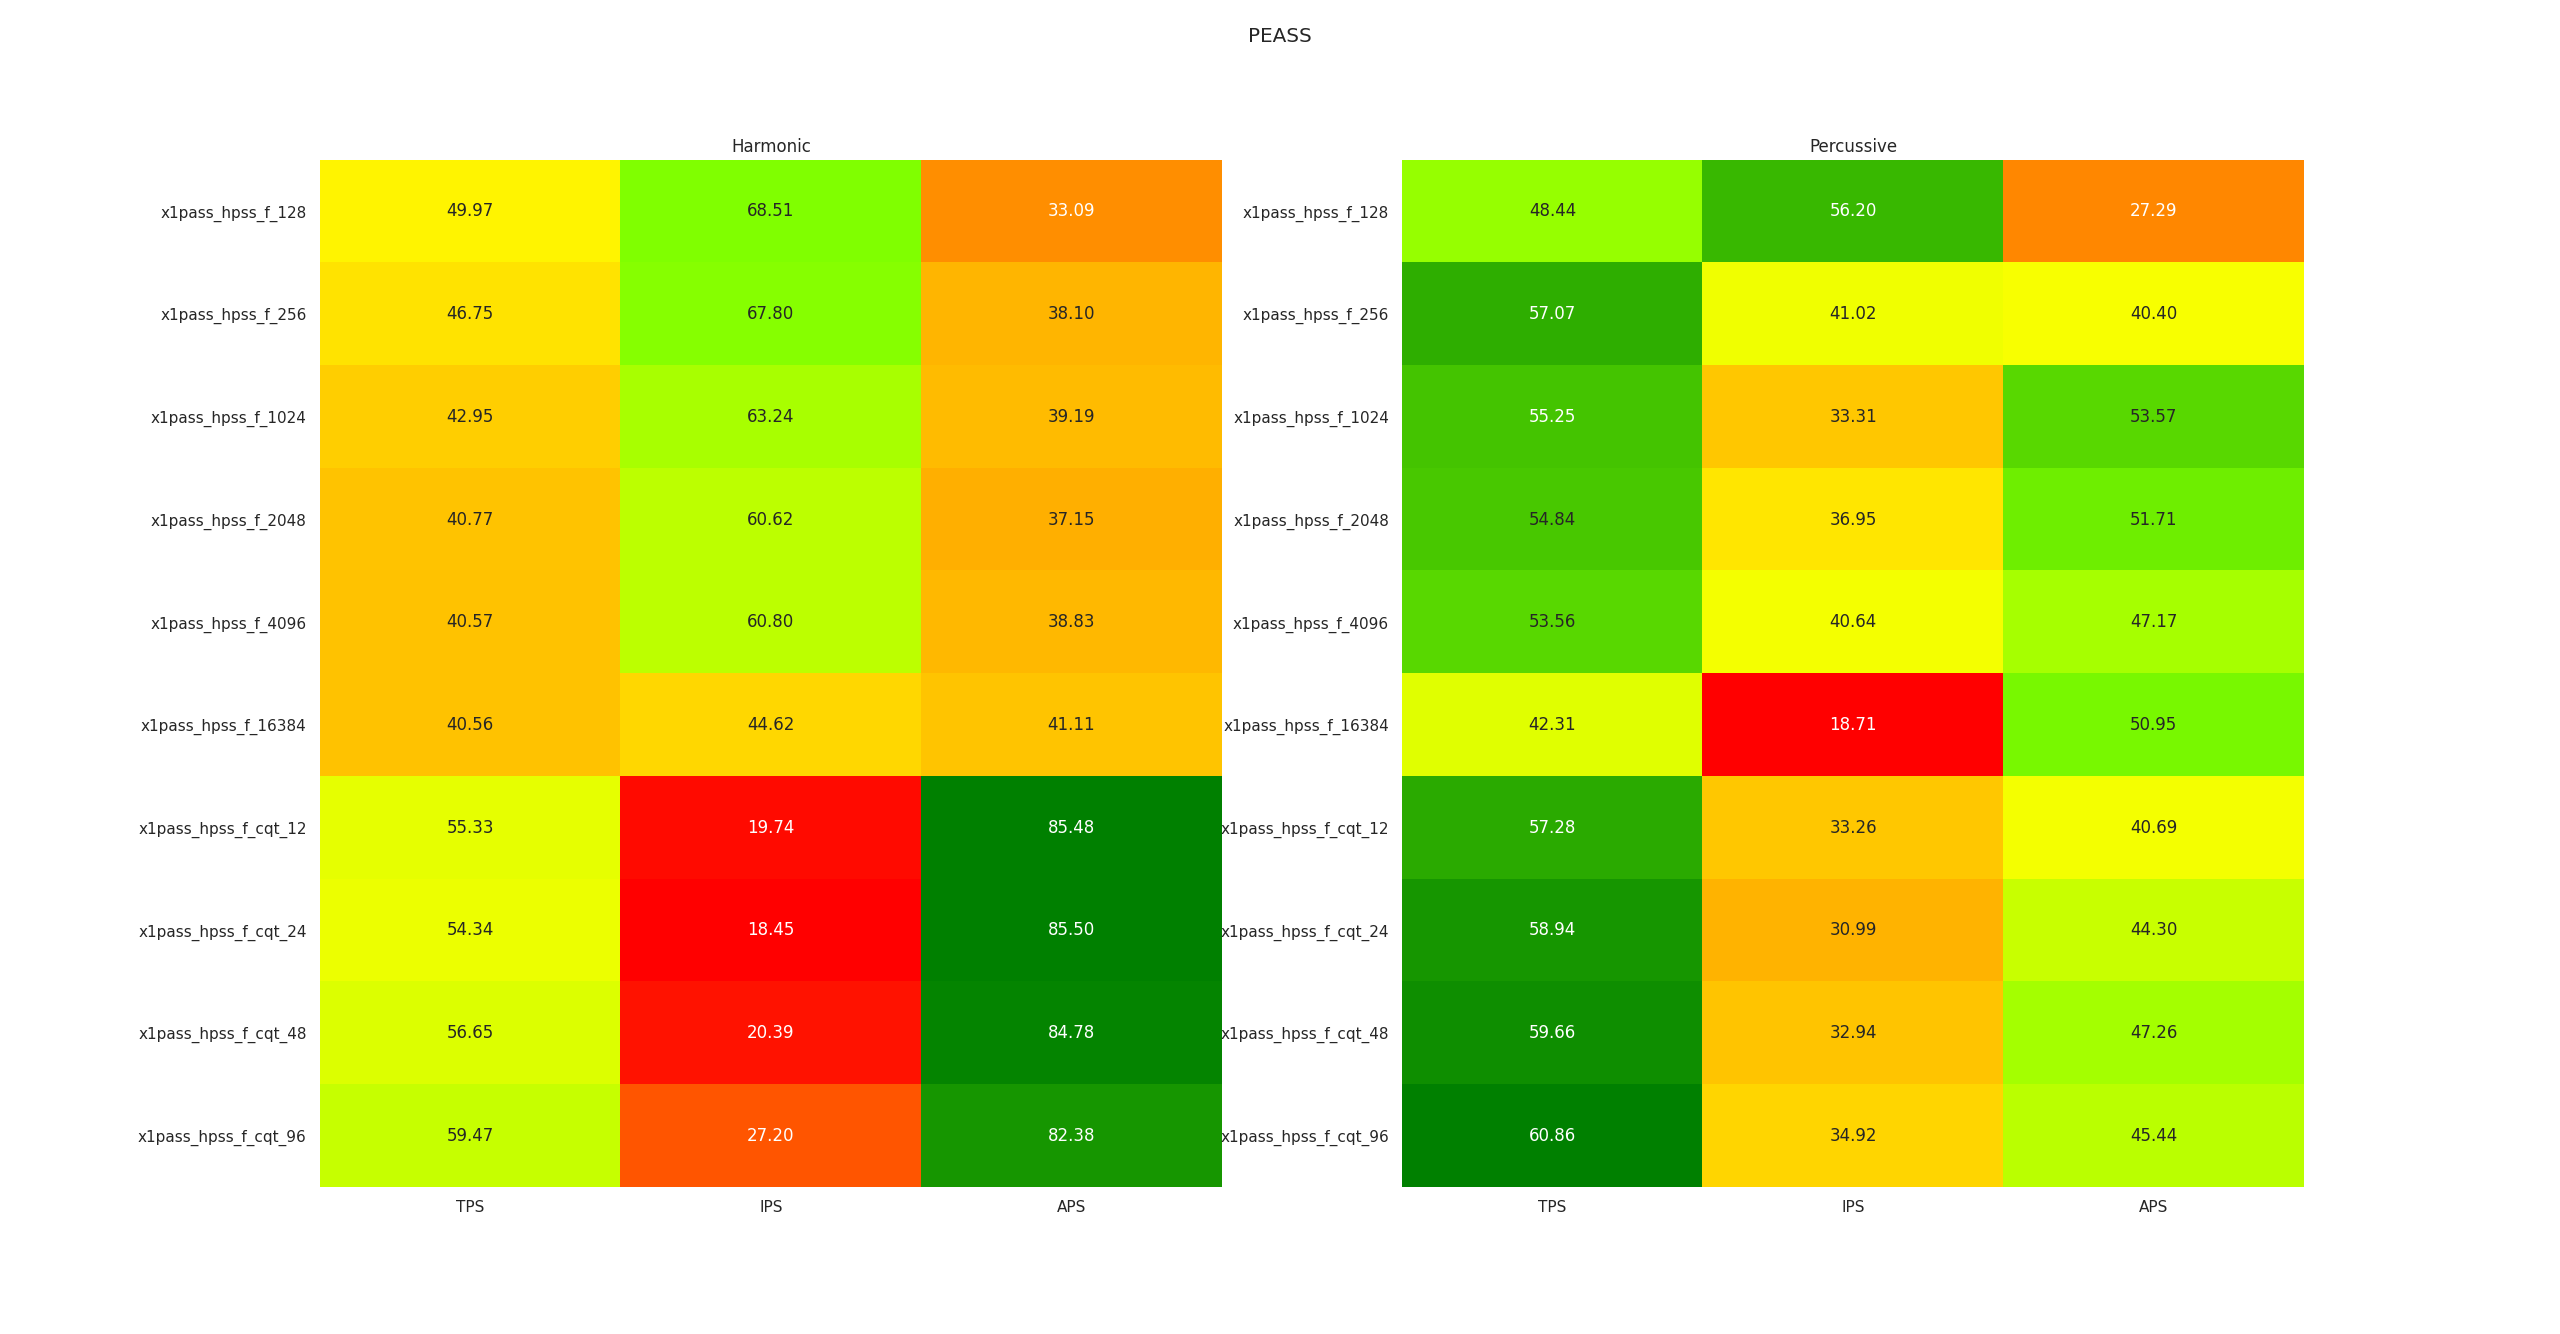
\includegraphics[width=20cm]{../evaluation/heatmaps/1pass_Fitzgerald_PEASS_abbrev.png}}
	\vspace{-1.25em}
	\caption{One-pass soft-masking PEASS results}
	\label{fig:round1soft}
\end{figure*}

\begin{figure*}
	\centering
	\vspace{-0.8em}
	\makebox[\textwidth]{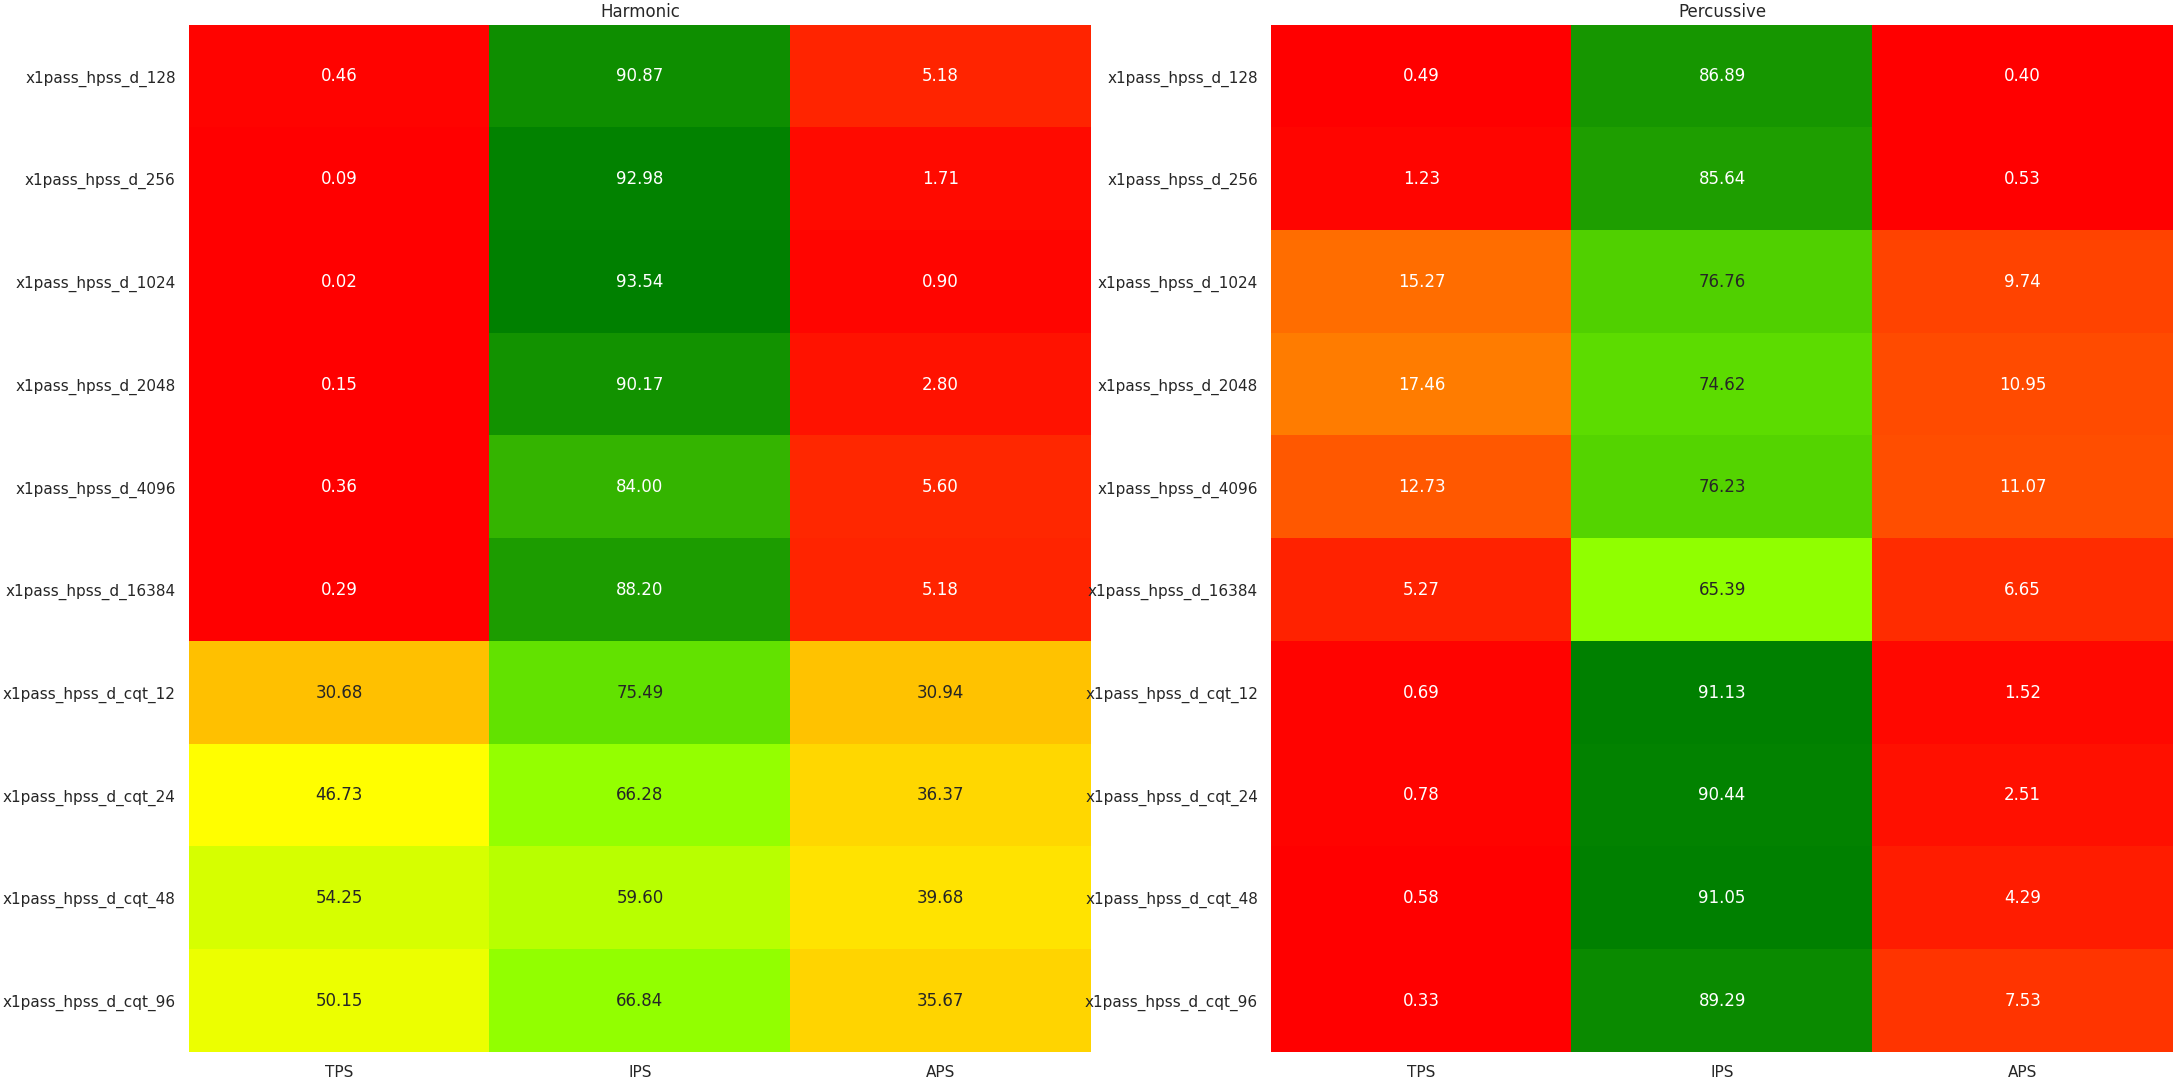
\includegraphics[width=20cm]{../evaluation/heatmaps/1pass_Driedger_PEASS_abbrev.png}}
	\vspace{-1.25em}
	\caption{One-pass hard-masking PEASS results}
	\label{fig:round1hard}
\end{figure*}

\subsubsection{Two-pass algorithms}

\citet{driedger}'s iterative algorithm is presented for harmonic/percussive source separation. The pseudocode is shown in Listing \ref{code:twopassdriedgerpseudo}.

\begin{listing}[h]
\setlength\partopsep{-\topsep}
\begin{minted}[numbersep=\mintednumbersep,linenos,mathescape=true,breaklines,frame=single,escapeinside=||]{text}
|$s = \text{mixed audio}$|
|$\hat{S1} = \text{STFT}(s, \text{window\_size}=4096)\text{\textbf{ or CQT}}$|
|$S1 = \text{abs}(\hat{S1})$|
|$H1 = \text{medianfilter}(S1, l_{H}, \text{axis}=2)$|
|$P1 = \text{medianfilter}(S1, l_{P}, \text{axis}=1)$|
|$ M_{H1} = \frac{H1}{P1 + \epsilon} \ge \beta $|
|$ M_{P1} = \frac{P1}{H1 + \epsilon} > \beta$|
|$\hat{H1} = \hat{S1} \cdot M_{H1}$|
|$\hat{P1} = \hat{S1} \cdot M_{P1}$|
|$\text{\textbf{final harmonic} }h1 = \text{ISTFT}(\hat{H1})\text{\textbf{ or ICQT}}$|
|$\text{\textbf{next input        } } p1 = \text{ISTFT}(\hat{P1})\text{\textbf{ or ICQT}}$|
|$\hat{S2} = \text{STFT}(p1, \text{window\_size}=256)\text{\textbf{ or CQT}}$|
|$S2 = \text{abs}(\hat{S2})$|
|$H2 = \text{medianfilter}(S2, l_{H}, \text{axis}=2)$|
|$P2 = \text{medianfilter}(S2, l_{P}, \text{axis}=1)$|
|$ M_{H2} = \frac{H2}{P2 + \epsilon} \ge \beta $|
|$ M_{P2} = \frac{P2}{H2 + \epsilon} > \beta$|
|$\hat{H1} = \hat{S2} \cdot M_{H2}$|
|$\hat{P1} = \hat{S2} \cdot M_{P2}$|
|$h2 = \text{ISTFT}(\hat{H2})\text{\textbf{ or ICQT}}$|
|$\text{\textbf{final percussive} } p2 = \text{ISTFT}(\hat{P2})\text{\textbf{  or ICQT}}$|
\end{minted}
\caption{Two-pass median-filtering HPSS pseudocode, hard mask}
\label{code:twopassdriedgerpseudo}
\end{listing}

The conclusions from the previous round of testing are used to prepare 3 variants of two-pass hard masking HPSS:
\begin{tight_enumerate}
	\vspace{-0.5em}
	\item
		The first variant uses STFT-16384 in the first pass, and STFT-2048 in the second pass (the best performing STFT configurations for harmonic and percussive separation, respectively).
	\item
		The second variant uses CQT-96 in the first pass for the harmonic separation (top harmonic performer), and STFT-2048 (top percussive performer) in the second pass.
	\item
		The third variant is the default with the exact settings (STFT-4096 for harmonic, STFT-256 for percussive) from the paper (\cite{driedger}).
\end{tight_enumerate}

The results in \ref{fig:round2hard} show that the CQT-96/STFT-2048 algorithm performs the best. By the PEASS evaluation, the target and artifact scores for the CQT-96/STFT-2048 variant are better, at the expense of a slightly lower interference score.

\begin{figure*}
	\centering
	\vspace{-0.8em}
	\makebox[\textwidth]{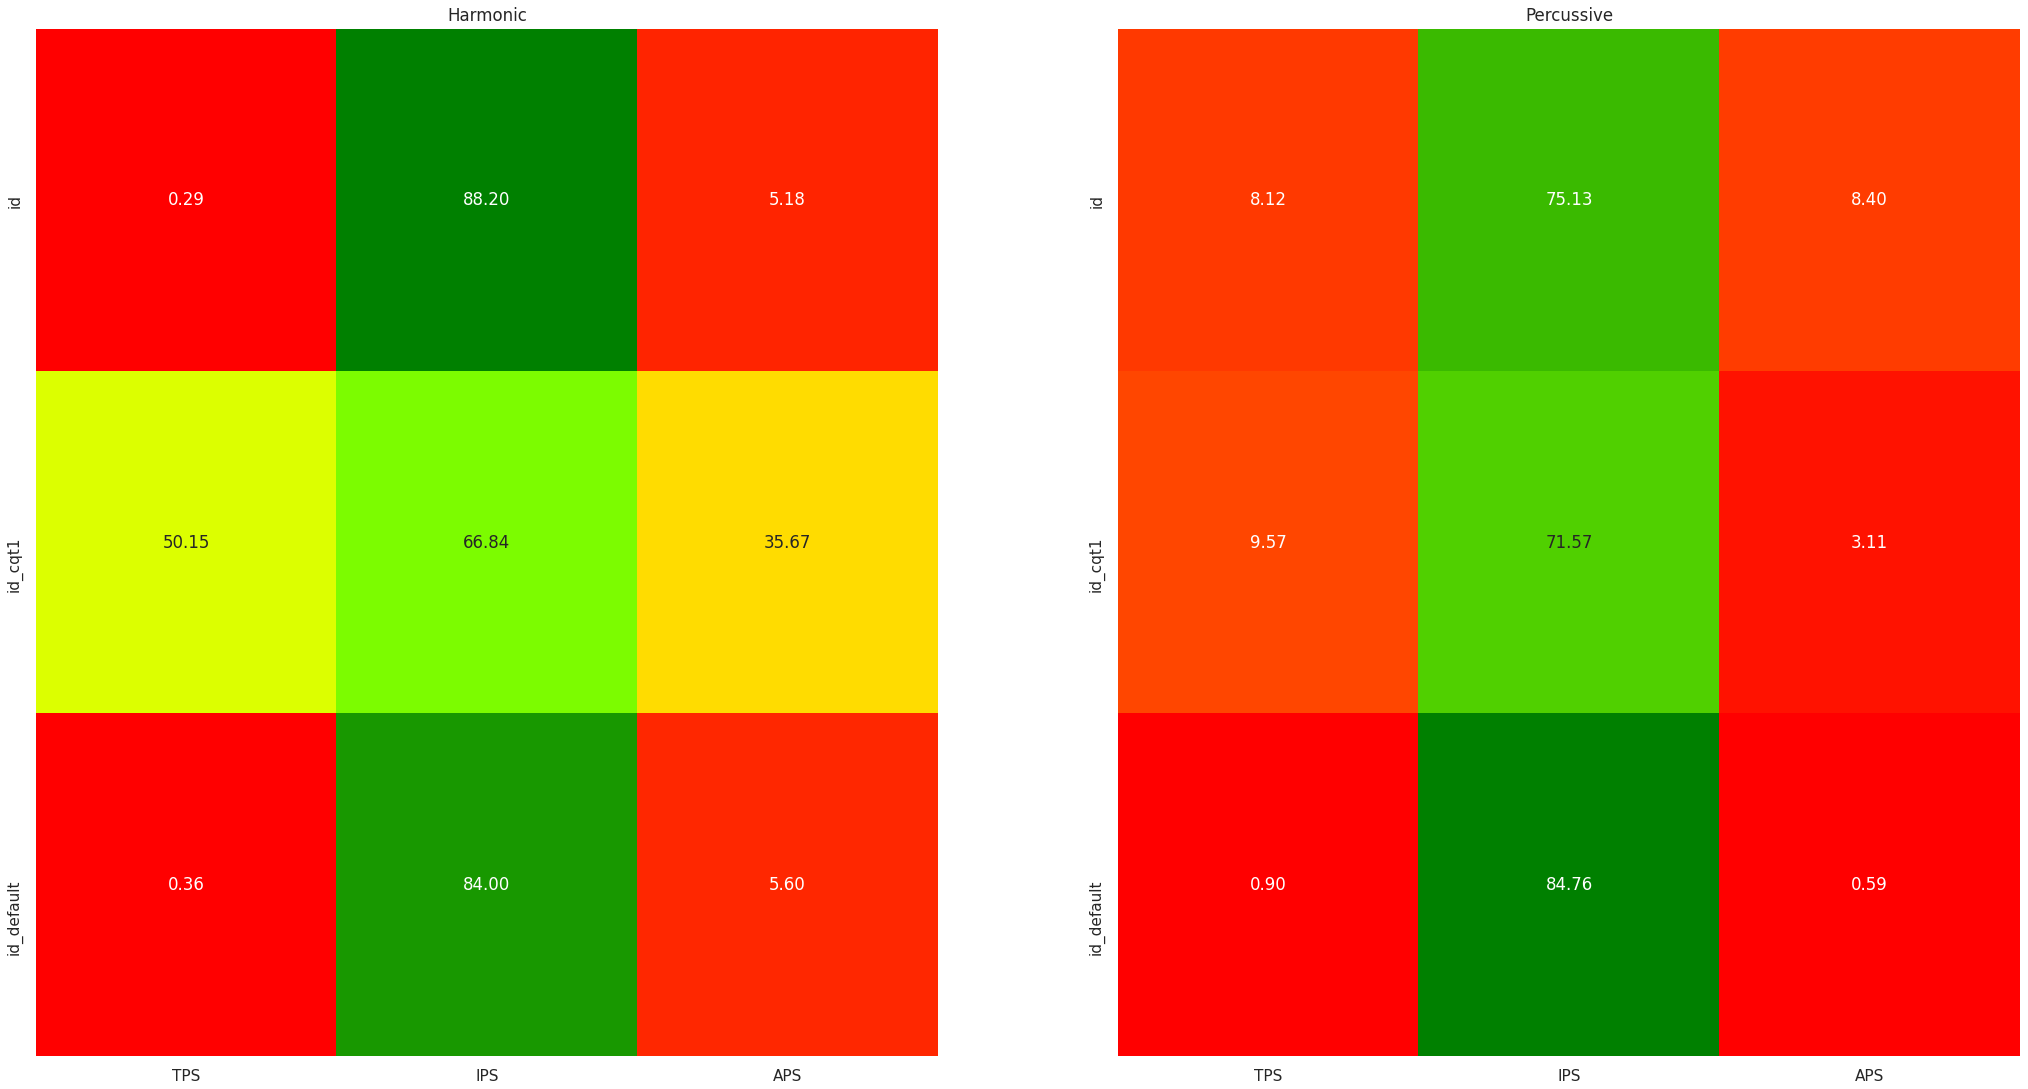
\includegraphics[width=16cm]{../evaluation/heatmaps/2pass_Driedger_PEASS_abbrev.png}}
	\vspace{-1.25em}
	\caption{Two-pass hard-masking PEASS results}
	\label{fig:round2hard}
\end{figure*}

%%%%%%%%%%%%%%%%%%%%%
% HYBRID ALGORITHMS %
%%%%%%%%%%%%%%%%%%%%%
\section{Hybrid algorithms}
\label{sec:hybrids}

\vfill
\clearpage % force a page break before references

\nocite{*}
\printbibheading[title={References}]
\printbibliography[heading=none]

\end{document}
